\section{Thiết kế kiến trúc}
    \subsection{Thiết kế cơ sở dữ liệu của hệ thống}
        \subsubsection{Biểu đồ EERD}
            \begin{figure}[H]
            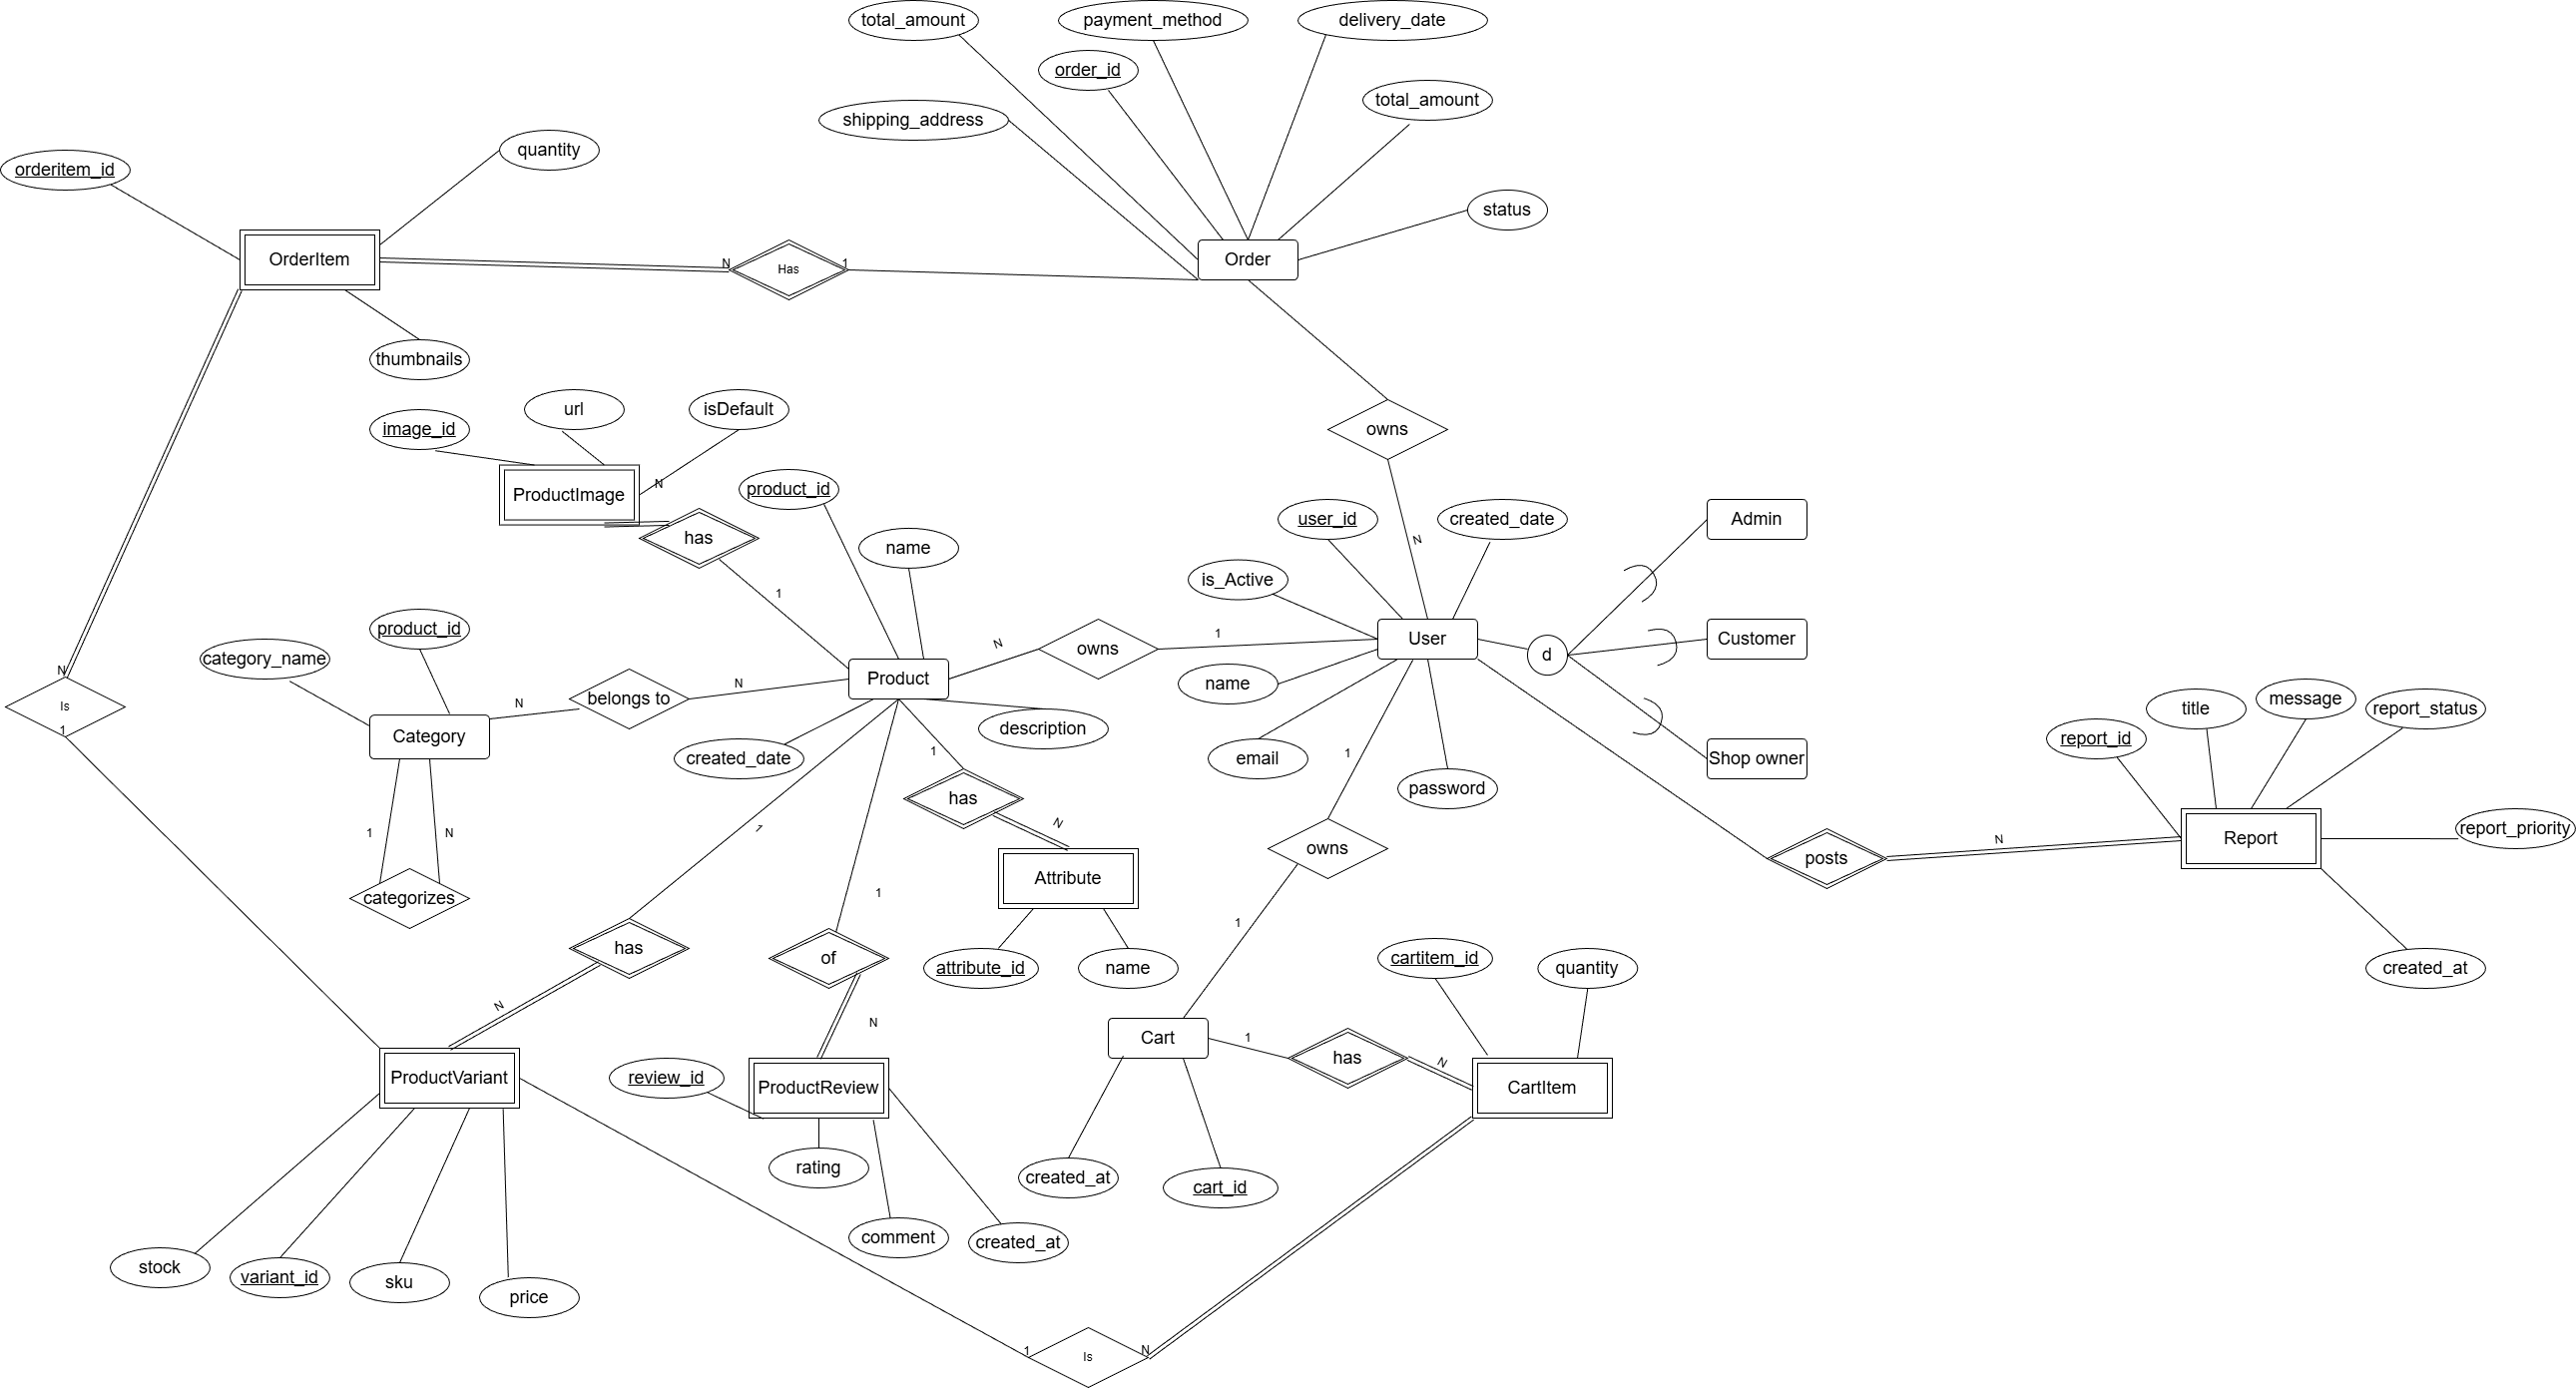
\includegraphics[width=\textwidth, keepaspectratio] {image/EERD.drawio.png}
            \label{fig:enter-label}
            \caption{Biểu đồ EERD của hệ thống}
            \end{figure}
        \subsubsection{Lược đồ quan hệ}
            \begin{figure}[H]
            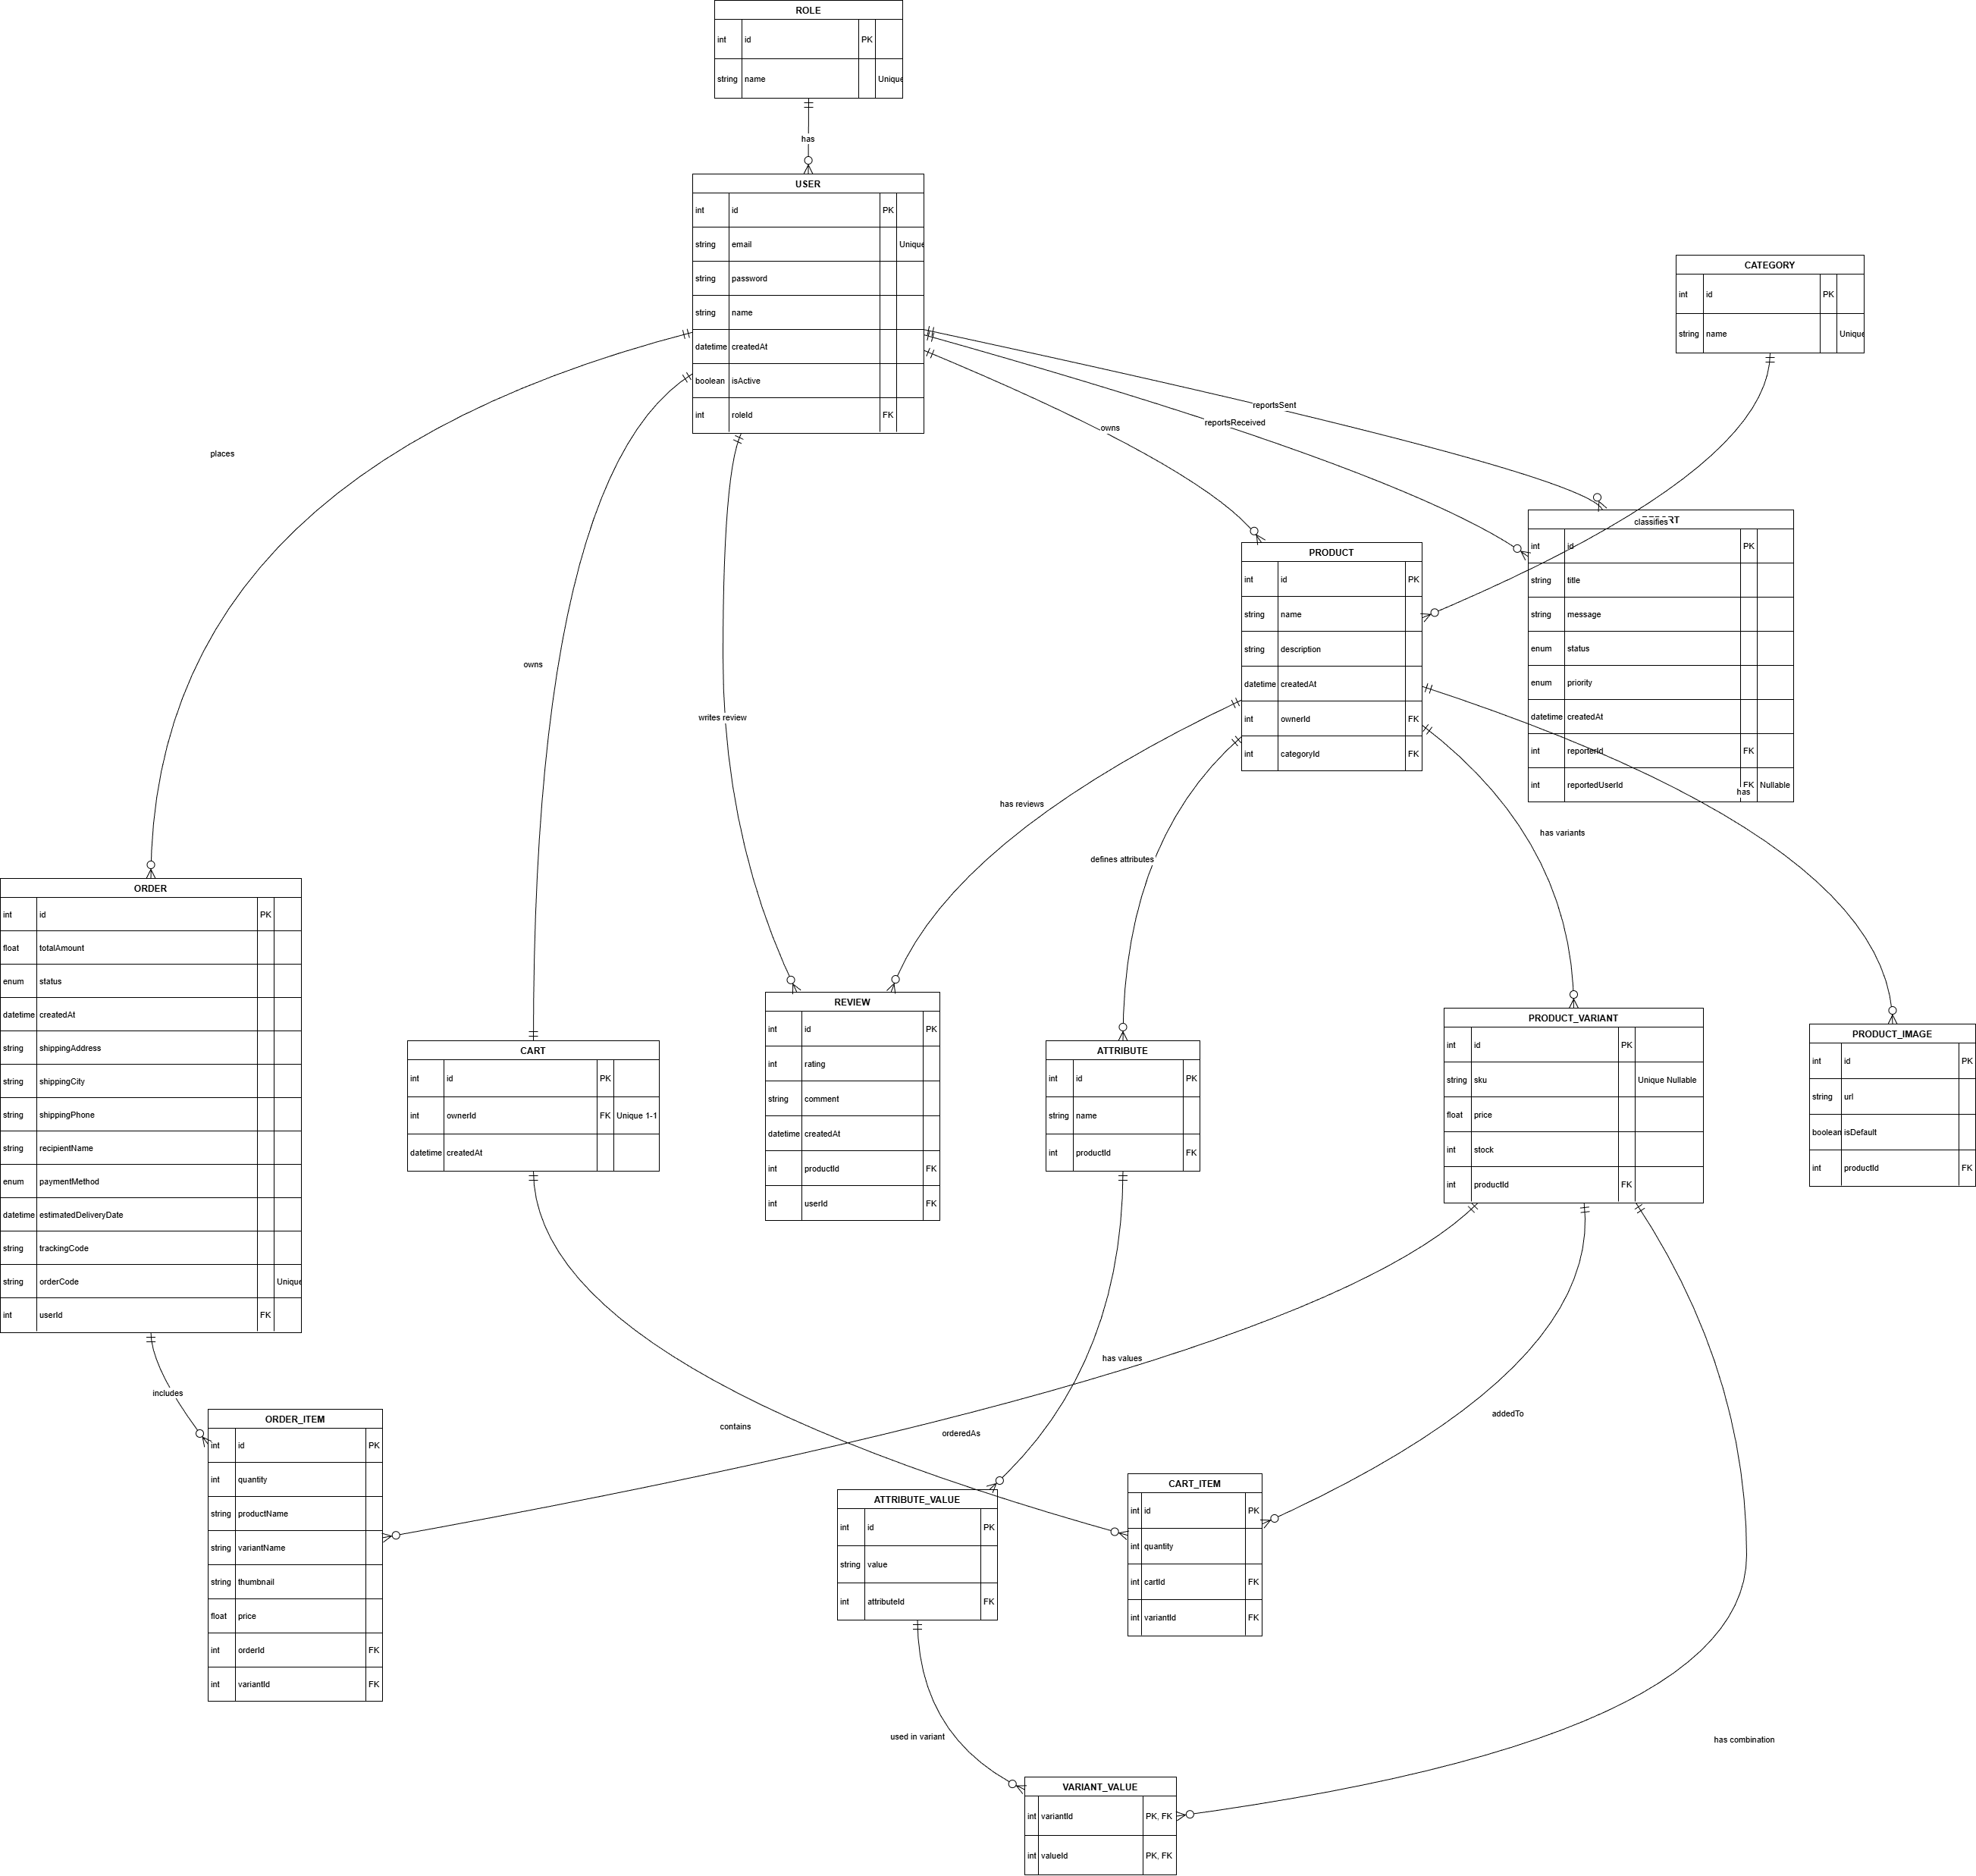
\includegraphics[width=\textwidth, keepaspectratio] {image/MAPPING.drawio.png}
            \label{fig:enter-label}
            \caption{Lược đồ quan hệ của hệ thống}
            \end{figure}
    \subsection{Phương pháp kiến trúc để triển khai hệ thống}

Sử dụng kiến trúc \textbf{MVC (Model-View-Controller)} kết hợp với kiến trúc \textbf{Client-Server} (Frontend - Backend tách biệt) để triển khai hệ thống VESTRA E-Commerce. Kiến trúc này phù hợp với công nghệ PERN Stack (PostgreSQL, Express, React, Node.js) vì:

\begin{itemize}
    \item \textbf{Tính phân tách rõ ràng:} Giúp chia tách biệt lớp giao diện người dùng (Frontend - View) và lớp xử lý logic/dữ liệu (Backend - Controller \& Model).
    \item \textbf{Quản lý dữ liệu phức tạp:} Với sự hỗ trợ của Prisma ORM, các thực thể phức tạp được mô hình hóa chặt chẽ.
    \item \textbf{Tăng tính linh hoạt và mở rộng:} Dễ dàng tích hợp thêm dịch vụ bên thứ 3 (như VNPAY) mà không làm vỡ cấu trúc.
    \item \textbf{Bảo mật và Hiệu năng:} Controller kiểm soát luồng dữ liệu, xác thực JWT và bảo vệ endpoint.
\end{itemize}

\vspace{0.5cm} % Tạo khoảng cách nhỏ cho thoáng
\noindent \textbf{Triển khai chi tiết vào hệ thống:}

% --- MODEL ---
\subsubsection*{1. Model (Mô hình)}
\begin{itemize}
    \item \textit{Chức năng:} Model chịu trách nhiệm quản lý cấu trúc dữ liệu, các ràng buộc và tương tác trực tiếp với cơ sở dữ liệu PostgreSQL thông qua Prisma ORM.
    \item \textit{Áp dụng trong hệ thống:}
        \begin{itemize}
            \item Các thực thể trong \texttt{schema.prisma}: \textbf{User} (Admin, Shop, User), \textbf{Product} (ProductVariant, Attribute), \textbf{Order}, \textbf{Cart} và \textbf{Report},...
            \item Mỗi thực thể trong ERD sẽ tương ứng với một lớp Model trong MVC, nơi định
 nghĩa các thuộc tính và phương thức để giao tiếp với cơ sở dữ liệu.
        \end{itemize}
\end{itemize}

% --- VIEW ---
\subsubsection*{2. View (Giao diện người dùng)}
\begin{itemize}
    \item \textit{Chức năng:} Hiển thị dữ liệu và tiếp nhận tương tác. Sử dụng \textbf{React}, \textbf{Vite} và \textbf{Material UI}.
    \item \textit{Áp dụng trong hệ thống:}
        \begin{itemize}
            \item \textbf{User Dashboard:} Trang chủ, Tìm kiếm, Giỏ hàng, Checkout.
            \item \textbf{Shop Dashboard:} Quản lý sản phẩm, biến thể, kho hàng; quản lý đơn hàng.
            \item \textbf{Admin Dashboard:} Quản lý người dùng, báo cáo, khiếu nại.
            \item Gọi API đến Backend để lấy JSON và render giao diện responsive.
        \end{itemize}
\end{itemize}

% --- CONTROLLER ---
\subsubsection*{3. Controller (Điều khiển)}
\begin{itemize}
    \item \textit{Chức năng:} \textbf{Node.js + Express} đóng vai trò trung tâm xử lý logic. Tiếp nhận Request, xác thực, gọi Model và trả về Response.
    \item \textit{Áp dụng trong hệ thống:}
        \begin{itemize}
            \item \textbf{Xử lý đơn hàng:} Tính tổng tiền, tạo Order, tích hợp cổng thanh toán \textbf{VNPAY} (Redirect/IPN).
            \item \textbf{Xác thực \& Phân quyền:} Kiểm tra JWT token để phân quyền Admin/Shop/User.
            \item \textbf{Quản lý luồng dữ liệu:} Validate dữ liệu đầu vào từ Form trước khi lưu xuống DB.
        \end{itemize}
\end{itemize}